% !TeX TXS-program:compile = txs:///pdflatex/[--shell-escape]

\documentclass[11pt, letterpaper]{article}

\usepackage{minted}
\usepackage[utf8]{inputenc}
\usepackage[T1]{fontenc}
\usepackage{lmodern}
\usepackage{graphicx}
\usepackage{longtable}
\usepackage{wrapfig}
\usepackage{rotating}
\usepackage{amsmath}
\usepackage{textcomp}
\usepackage{amssymb}
\usepackage{hyperref}
\usepackage[round]{natbib}
\usepackage{subcaption}


\title{\bfseries Tarea}
\author{Ángel García Báez}
\date{\today}
\setcounter{tocdepth}{3} 

\begin{document}
	
	% Página de presentación
	\begin{titlepage}
		\centering
		\includegraphics[width=0.2\textwidth]{logo.png}\par
		\vspace{1cm}
		{\LARGE \bfseries Universidad Veracruzana \par}
		\vspace{1cm}
		{\Large Maestría en Inteligencia Artificial\par}
		\vspace{3cm}
		{\LARGE \bfseries Visión por Computadora \par}
		\vspace{1cm}
		{\Large \bfseries Examen 2. Segmentación y trnasformada de Hough \par}
		\vfill
		{\Large \textit{Ángel García Báez}\par}
		\vspace{1cm}
		{\Large Profesor: Dr. Héctor Acosta Mesa \par}
		\vfill
		{\Large \today \par}
	\end{titlepage}
	
	% Página exclusiva para la tabla de contenidos
	\newpage
	\tableofcontents
	\newpage
	
% Sección para el problema 1
\section{Ejercicio practico 1}

Se tiene la siguiente imagen y se quiere poder segmentar en sus 3 colores principales predominantes (los cuales se observan que son rojo, verde y blanco).



\begin{figure}[h!]
	\centering
	\begin{minipage}{0.8\textwidth}
		\centering
		\includegraphics[width=\textwidth]{IMG/G1.jpg}
		\caption*{Imagen 1. Verduras con colores muy marcados.}
	\end{minipage}\hfill
\end{figure}

Como propuesta para realizar dicha segmentación, se propone usar los pixeles de la imagen dentro del espacio de colores RGB y usar esos datos para realizar un proceso de agrupación por K-medias, donde de antemano se quieren obtener 3 grupos, por lo que el K es igual a 3. Esto se propone así por su sencillez de implementación y porque los colores de la imagen se muestran muy bien delimitados, es decir, no es muy compleja la composición de la imagen.

\newpage

A continuación se muestra el resultado de aplicar este proceso con k = 3 y coloreando los pixeles de la imagen con el color del centroide del grupo al que corresponden.

\begin{figure}[h!]
	\centering
	\begin{minipage}{0.8\textwidth}
		\centering
		\includegraphics[width=\textwidth]{IMG/R1.png}
		\caption*{Imagen 1. Verduras con colores muy marcados.}
	\end{minipage}\hfill
\end{figure}

Se observa que el resultado de la segmentación cumple su propósito, logra diferenciar bien los chiles y los tallos de los tomates, diferencia bien el fondo de las verduras pero con algunos pequeños errores que convierte el fondo como si fuera de color verde.

\newpage

\section{Ejercicio practico 2}

Se tiene la siguiente imagen de una pista de aterrizaje, de la cual se quiere extraer los bordes que delimitan a la misma mediante la transformada de Hough.


\begin{figure}[h!]
	\centering
	\begin{minipage}{0.7\textwidth}
		\centering
		\includegraphics[width=\textwidth]{IMG/G2.jpg}
		\caption*{Imagen 2. Pista de aterrizaje.}
	\end{minipage}\hfill
\end{figure}

Para llevar a cabo este proceso, primero fue necesario convertir la imagen en escala de blanco y negro para hacer la detección de bordes con el filtro de Canny.

\begin{figure}[h!]
	\centering
	\begin{minipage}{0.7\textwidth}
		\centering
		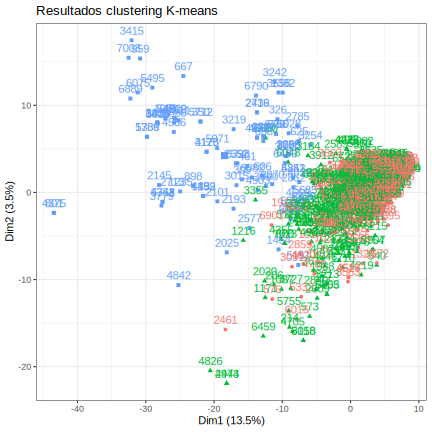
\includegraphics[width=\textwidth]{IMG/R2.png}
		\caption*{Pista con bordes detectados.}
	\end{minipage}\hfill
\end{figure}

\newpage

Posteriormente, se hicieron las estimaciones de los parametros de la ecuación del modelo de Hough para mandar los pixeles al espacio de Hough y detectar los picos más altos:


\begin{figure}[h!]
	\centering
	\begin{minipage}{0.7\textwidth}
		\centering
		\includegraphics[width=\textwidth]{IMG/R3.png}
		\caption*{Espacio de Hough.}
	\end{minipage}\hfill
\end{figure}

\begin{figure}[h!]
	\centering
	\begin{minipage}{0.7\textwidth}
		\centering
		\includegraphics[width=\textwidth]{IMG/R4.png}
		\caption*{Picos detectados.}
	\end{minipage}\hfill
\end{figure}

\newpage

Finalmente, con los picos detectados, se proyectan sobre la imagen original para mostrar las formas encontradas que delimitan a la pista de aterrizaje.

\begin{figure}[h!]
	\centering
	\begin{minipage}{0.7\textwidth}
		\centering
		\includegraphics[width=\textwidth]{IMG/R5.png}
		\caption*{Pista con los margenes proyectados.}
	\end{minipage}\hfill
\end{figure}






%\bibliographystyle{apalike}  % Estilo de citas (puedes cambiarlo)
%\bibliography{Biblio}        % Nombre del archivo BibTeX (sin extensión)

\newpage
	
\section{Anexos}	

\subsection{Implementación en matlab para la resolución de los ejercicios 1 y 2}


\begin{minted}[linenos,firstnumber=1]{matlab}

%% Cargar la imagen de las verduras %%
I = imread("imagen1.jpg");
imshow(I)

%% Pedir un kmeans con k = 3 %%
[seg,centros] = imsegkmeans(I,3);
imagesc(seg);
title("Imagen segmentada")
% Agregar los colores de los centros como el colormap %
colormap(centros);


%% Cargar la imagen para el segundo ejercicio %%
I = imread("imagen2.jpg");
imshow(I)

%% Convertir la imagen en escala de grises %%
BI = rgb2gray(I);

%% Aplicar la transformada con canny y volver a proyectar
BW = edge(BI,'canny');
imshow(BW);
title('Bordes detectados con Canny');

%% 4. Realizar la Transformada de Hough y proyectar su espacio %%
[H, T, R] = hough(BW);
imshow(imadjust(rescale(H)), 'XData', T, 'YData', R, ...
'InitialMagnification', 'fit');
title('Espacio de Hough');
xlabel('\theta (degrees)');
ylabel('\rho');
axis on, axis normal, hold on;
colormap(gca, hot); 



%% 5. Encontrar los picos en el espacio de Hough
P = houghpeaks(H, 5, 'threshold', ceil(0.6 * max(H(:))));
x = T(P(:,2));
y = R(P(:,1));
plot(x, y, 's', 'Color', 'black');

%% 6. Extraer las líneas de los picos encontrados
lines = houghlines(BW, T, R, P, 'FillGap', 20, 'MinLength', 40);
imshow(I); % Muestra la imagen original
title('Líneas de la pista de aterrizaje detectadas');
hold on; % Permite dibujar sobre la imagen
max_len = 0; % Para encontrar la línea más larga, opcional
for k = 1:length(lines)
xy = [lines(k).point1; lines(k).point2];
plot(xy(:,1), xy(:,2), 'LineWidth', 2, 'Color', 'red'); % Dibuja la línea en rojo
% Marca los puntos inicial y final de la línea (opcional)
plot(xy(1,1), xy(1,2), 'x', 'LineWidth', 2, 'Color', 'yellow');
plot(xy(2,1), xy(2,2), 'x', 'LineWidth', 2, 'Color', 'green');
% Determina la línea más larga (opcional)
len = norm(lines(k).point1 - lines(k).point2);
if ( len > max_len)
max_len = len;
longest_line = xy;
end
end
if exist('longest_line', 'var')
plot(longest_line(:,1), longest_line(:,2), 'LineWidth', 2, 'Color', 'blue');
end
hold off;

\end{minted}

\end{document}

